

\chapter{Stand der Wissenschaft und Technik}\label{cha:2}

Zur Abbildung geeigneter Welleneigeschaften in einer Messkabine, die selbst ebenfalls möglichst wenig Beeinflussung durch äußere Felder erfährt, ist ein grundlegendes Verständnis elektrischer und magnetischer Felder, sowie deren Ausbreitung im Raum und Interaktion mit unterschiedlichen Grenzschichten notwendig. Weiterhin soll die Schirmdämpfung als zu messende Größe der CNT-Folien allgemein betrachtet werden, sodass im Anschluss daran verschiedene Möglichkeiten der Messung vorgestellt werden können. \par
\vspace{\linespace}
Mithilfe der Theorie der Eigenschaften von Wellenfeldern wird dann aus betrachteten Messmethoden die ausgewählt, mit der sich die Anforderungen an die durchzuführende Vermessung von Schirmmaterialien bestmöglich erfüllen lassen. Die wissenschaftlichen Grundlagen dienen weiterhin als Basis für die Detailkonstruktion der Messkabine.


\section{Grundlagen elektromagenetischer Wellenfelder}\label{cha:2_Grundlagen}


Allgemein beschreibt ein Feld die Gesamtmenge aller Werte einer physikalischen Größe, die allen Punkten eines leeren oder stoffgefüllten Raumes zugeordnet sind, die sogenannte Feldgröße \cite{Spektrum.de_Feld}. Je nach Art der Feldgröße wird der allgemeine Feldbegriff in Skalarfeld 

\begin{equation}
    a(x,y,z, \ldots)    
\end{equation}


und Vektorfeld 

\begin{equation}
    \vec A(x,y,z,\ldots)
\end{equation}

unterteilt. Durch die Darstellung der Abhängigkeit von den Ortskoordinaten des Raumes wird deutlich, dass es sich bei einer Größe um ein Feld handelt. \par
\vspace{\linespace}
Die im Rahmen dieser Arbeit wichtigen Felder sind das elektrische und das magnetische Feld. Eine Beschreibung des Zusammenhanges zwischen der Feldursache und dem entstehenden Feld lässt sich in beiden Fällen mithilfe der Materialgleichungen und der Maxwell'schen Gleichungen vornehmen~\cite{EM_Schirmung}. Grundlegend lässt sich ein Feld jedoch auch ohne Kenntnis seiner Ursache beschreiben, sodass im Rahmen dieser Arbeit nicht explizit auf die Maxwell'schen Gleichungen eingegangen werden soll, da dies thematisch zu weit führen würde. 


\subsection{Elektrisches Feld}\label{cha:2_sub_Elektrisches_Feld}

Um das elektrische Feld mittels seiner Wirkungs zu beschreiben, wird eine Testladung in das Feld eingebracht, auf die daraufhin eine Kraft $\vec F_q(x,y,z,q)$ wirkt. Da die Kraft eine gerichtete Größe ist, muss die Beschreibung des elektrischen Feldes mittels eines Vektorfeldes beschrieben werden. Die Größe der Kraft ist abhängig von der eingebrachten Ladung. Um eine Veränderung des Feldes durch die Testladung auszuschließen, wird stattdessen eine infinitesimale Teilladung $dq$ zur Beschreibung des Feldes verwendet, was sich damit aus

\begin{equation}
    \vec E (x,y,z) = \frac{d\vec F_q(x,y,z,q)}{dq}
\end{equation}

ergibt. Der Differentialquotient $\vec E$ ist die elektrische Feldstärke \cite{EM_Schirmung}. \par
\vspace{\linespace}
Damit ist die Wirkung eines elektrischen Feldes beschrieben, jedoch noch nicht dessen Ursache. Nach dem sogenannten Satz des Hüllenflusses, dem ersten Maxwell'schen Gesetz, erfahren Ladungen nicht nur Beeinflussung durch ein elektrisches Feld, sondern sind auch dessen Ursache. Eine Beschreibung kann am einfachsten mithilfe eines Plattenkondensators erfolgen, dessen Plattenflächen $A_P$ senkrecht auf den Feldlinien eines elektrisches Feldes stehen und auf welche die Ladungen $+q$ und $-q$ genau so aufgebracht werden, dass im Inneren des Kondensators das äußere Feld kompensiert wird. Eine von der Fläche unabhängige Größe zur Beschreibung des elektrischen Feldes lässt sich wiederum durch den Differentielquotienten 

\begin{equation}
    \vec D(x,y,z) = \frac{dq}{dA_P} \cdot \vec n_A
\end{equation}

erhalten, der elektrischen Flussdichte $\vec D$ \cite{EM_Schirmung}. \par
\vspace{\linespace}

Da sowohl die Feldstärke als auch die Flussdichte das elektrische Feld beschreiben, gibt es in Abhängigkeit Materials, aus dem der felderfüllte Raum besteht, einen Zusammenhang zwischen beiden Größen, die sogenannte Dielektrizitätszahl oder Permittivität $\varepsilon$, die eine Materialeigenschaft ist. Es gilt

\begin{equation}
    \vec D = \varepsilon \cdot \vec E = \varepsilon_0 \varepsilon_r \cdot \vec E \qquad \quad \text{mit} \qquad \varepsilon_0 = 8,85419 \cdot 10^{-12} \; \si{\ampere\second\per\volt\per\meter}
    \label{eq:2_Materialgleichung_elektrisches_Feld}
\end{equation}

mit der Dielektrizitätszahl des leeren Raumes $\varepsilon_0$ und der relativen Dielektrizitätszahl $\varepsilon_r$ des betrachteten Materials \cite{EM_Schirmung}.


\subsection{Magnetisches Feld}\label{cha:2_sub_Magnetisches_Feld}

Wie auch die elektrische Feldstärke wird die magnetische Flussdichte indirekt beschrieben, d.h. über ihre messbare Kraftwirkung auf elektrische Ströme bzw. bewegte Ladungen. Dabei wird ein stromdurchflossener Draht der Länge $L$ so über einem Magnetfeld angeordnet, dass die messbare Kraft maximal wird. Um auch hier Rückwirkungen auszuschließen, wird eine differentielle Drahtlänge, die vom infinitesimal kleinen Strom $dI$ durchflossen wird, betrachtet. Mit des Differentialquotienten

\begin{equation}
    \vec B(x,y,z) = \frac{d^2 \vec F_L(x,y,z,L,I)}{dL \cdot dI}
\end{equation}

lässt sich die magentische Flussdichte, die sowohl vom Strom $I$ als auch von der Drahtlänge $L$ abhängt, aus der gemessenen Kraft ermitteln \cite{EM_Schirmung}. 
\par
\vspace{\linespace}
Analog zur Betrachtung elektrischer Felder lässt sich feststellen, dass Ströme nicht nur eine Kraftwirkung durch magnetische Felder erfahren, sondern auch deren Ursache sind. Dazu lässt sich ebenfalls ein einfaches Gedankenexperiment ähnlich der Betrachtung zur elektrischen Flussdichte durchführen: 
\par
\vspace{\linespace}
In einer Spule der Länge $L$ fließe ein Strom $I$, der genau so groß ist, dass durch die induzierte magnetische Flussdichte ein umgebendes äußeres Magnetfeld im Inneren der Spule verschwindet. Die Ausrichtung der Anordnung sei wiederum so erfolgt, dass der Strom $I$ maximal wird. Der erforderliche Strom ist abhängig von der Spulenlänge und deren Windungszahl $N_w$. Das Differential

\begin{equation}
    \vec H(x,y,z) = N_w \frac{dI(x,y,z,L)}{dL} \cdot \vec n_A
\end{equation}

beschreibt die magnetische Feldstärke, welche senkrecht auf der Spulenquerschnittsfläche steht \cite{EM_Schirmung}. 
\par
\vspace{\linespace}
Ebenso wie die elektrische Feldstärke und Flussdichte sind auch die beschreibenden Feldgrößen des magnetischen Feldes proportional zueinander und lassen sich über eine Materialkonstante, der sogenannten Permeabilität $\mu$, ineinander umrechnen:

\begin{equation}
    \vec B = \mu \cdot \vec H = \mu_0 \mu_r \cdot \vec H \qquad \quad \text{mit} \qquad \mu_0 = 4\cdot \pi \cdot 10^{-7} \; \si{\volt\second\per\ampere\per\meter}.
    \label{eq:2_Materialgleichung_magnetisches_Feld}
\end{equation}

Die relative Permeabilität $\mu_r$ ist ein Materialparameter und die Permeabilität des Vakuums $\mu_0$, ebenso wie $\varepsilon_0$, eine Naturkonstante \cite{EM_Schirmung}.
\par
\vspace{\linespace}
Eine Verknüpfung des elektrischen Feldes mit dem magnetischen kann über den ein einem Leiter hervorgerufenen Stromfluss erfolgen. Die verknüpfende Größe der erzeugten Stromdichte $\vec j$,

\begin{equation}
    \vec j = \sigma \cdot \vec E,
\end{equation}

ist dabei die Leitfähigkeit $\sigma$ des betrachteten Leitermaterials.


\subsection{Verhalten elektrischer und magnetischer Felder an Grenzflächen}

In den vorangegangenen \Abschnitten \ref{cha:2_sub_Elektrisches_Feld} und \ref{cha:2_sub_Magnetisches_Feld} wurde die Abhängigkeit der Flussdichte- und Feldstärkevektoren voneinandern mithilfe von Materialeigenschaften beschrieben. Breiten sich die Felder also entlang verschiedener Materialien mit unterschiedlichen Dielektrizitäten und Permeabilitäten aus, ändern sich beim Übergang zwangsläufig die Ausbreitungsbedingungen. Dies soll im Folgendes betrachtet werden, da das Verhalten der Felder an Materialgrenzflächen grundlegend für die Untersuchtung von Materialschirmen ist. 
\par
\vspace{\linespace}
Für die folgende Betrachtung sei angenommen, dass die untersuchte Grenzfläche relativ zum felderfüllten Raum eine allgemeine Lage aufweist und somit die jeweiligen Feldvektoren schräg auf die Grenzfläche auftreten (vgl. \Abb \ref{fig:2_Flussdichten_an_Grenzflaechen}). Weiterhin werden die Vektoren in der folgenden Untersuchung in ihre Normal- und Tangentialkomponente zur betrachteten Grenzfläche zerlegt, was jeweils durch die Indizes~$n$ und $t$ verdeutlicht wird. 

\begin{figure}[ht]
    \centering
    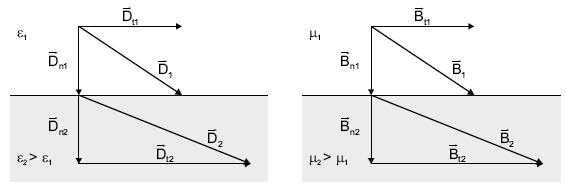
\includegraphics[width=0.75\textwidth]{Abbildungen/Kapitel2/Flussdichten_an_Grenzflaechen.png}
    \caption{Verhalten elektrischer und magnetischer Flussdichtevektoren an Grenzflächen von \mbox{Materialien} unterschiedlicher Dielektrizität bzw. Permeabilität}
    \label{fig:2_Flussdichten_an_Grenzflaechen}
\end{figure}

Beim Materialübergang von Flussdichtevektoren ist festzustellen, dass die Normalkomponenten an der Grenzfläche in beiden Materialien konstant sind (vgl. \Abb \ref{fig:2_Flussdichten_an_Grenzflaechen}) \cite{EM_Schirmung}.  

\begin{equation}
    \vec D_{n1} = \vec D_{n2}
\end{equation}
\begin{equation}
    \vec B_{n1} = \vec B_{n2}
\end{equation}


Aus den vorgestellten Materialgleichungen~\ref{eq:2_Materialgleichung_elektrisches_Feld} und \ref{eq:2_Materialgleichung_magnetisches_Feld} ergibt sich daraus für die Normalkomponenten der Feldstärke bei gleichbleibender Flussdichte zwangsläufig ein Sprung an der Grenzfläche im reziproken Verhältnis der Dielektrizitäten bzw. Permeabilitäten aufgrund der unterschiedlichen Materialeigenschaften. Somit gilt

\begin{equation}
    \vec E_{n1} = \frac{\varepsilon_2}{\varepsilon_1} \cdot \vec E_{n2} \\
\end{equation}
\begin{equation}
    \vec H_{n1} = \frac{\mu_2}{\mu_1} \cdot \vec H_{n2}
\end{equation}

für die Normalkomponenten der Feldstärken. Die Abbildung \ref{fig:2_Feldstaerken_an_Grenzflaechen} verdeutlicht dies. 

\begin{figure}[ht]
    \centering
    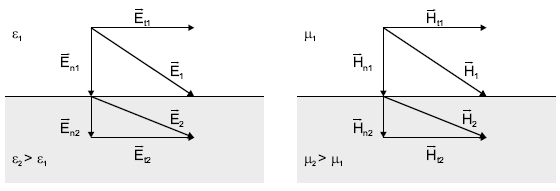
\includegraphics[width=0.75\textwidth]{Abbildungen/Kapitel2/Feldstaerken_an_Grenzflaechen.png}
    \caption{Verhalten elektrischer und magnetischer Feldstärkevektoren an Grenzflächen von \mbox{Materialien} unterschiedlicher Dielektrizität bzw. Permeabilität}
    \label{fig:2_Feldstaerken_an_Grenzflaechen}
\end{figure}

Betrachtet man die Feldursachen bzw. die beschreibenden Maxwell'schen Gleichungen wird offentlichtsicht, dass für die Vektoren der Feldstärke wiederum die Tangentialkomponente in beiden Materialien beim Übergang über die Grenzschicht gleich bleiben muss \cite{EM_Schirmung}. 

\begin{equation}
    \vec E_{t1} = \vec E_{t2}
\end{equation}
\begin{equation}
    \vec H_{t1} = \vec H_{t2}
\end{equation}

Mit einer ähnlichen Argumentation wie vorher kann gezeigt werden, dass damit für die tangentialen Komponenten der Flussdichtevektoren die Beziehungen

\begin{equation}
    \vec D_{t1} = \frac{\varepsilon_1}{\varepsilon_2} \vec D_{t2}
\end{equation}
\begin{equation}
    \vec B_{t1} = \frac{\mu_1}{\mu_2} \vec B_{t2}
\end{equation}

Damit gelten ebenfalls für die resultierenden Vektoren $\vec D_1$ und $\vec D_2$ bzw. $\vec B_1$ und $\vec B_2$ die Materialgesetze~\ref{eq:2_Materialgleichung_elektrisches_Feld} und \ref{eq:2_Materialgleichung_magnetisches_Feld}. Ein Sprung in den Materialeigenschaften äußert sich demnach in einer Brechung der resultierenden Feldlinien in Abhängigkeit der Verhältnisse $\varepsilon_1 / \varepsilon_2$ und $\mu_1 / \mu_2$, welche analog der Brechung von Licht beim Übergang in unterschiedliche optische Materialien veranschaulicht werden kann. Unter der Vorraussetzung isotroper Materialien hintsichtlicht Dielektrizität und Permeabilität gilt weiterhin, dass die resultierenden Flussdichte- und Feldstärkevektoren des elektrischen bzw. magnetischen Feldes in den jeweiligen Materialien kollinear sind und die gleiche Orientierung haben.

\par
\vspace{\linespace}

Für das Verständnis der Wirkungsweise von elektromagnetischen Schirmen ist dieses Verhalten von Feldern an Grenzflächen eine wichtige Grundvoraussetzung.




%Da Schirm für eindringende Wellen -> wichtig











\section{Wellenausbreitung}\label{cha:2_Wellenausbreitung}


\subsection{Entstehung einer elektromagnetischen Welle}\label{cha:2_sub_Entstehung_einer_Welle}

Die Entstehung einer elektromagnetischen Welle, ausgehend von einem Dipol beispielsweise, beruht auf der Wechselwirkung elektrischer und magnetischer Felder. Vereinfacht beschrieben führt ein Leitungsstrom zwischen einem Paar entgegengesetzter Ladungen (Dipol), zur Induktion eines Magnetfeldes, welches seinerseits wieder ein elektrischer Feld hervorruft. Im Verlauf des Ladungsausgleiches nimmt der Leitungsstrom und damit ebenfalls das Magnetfeld immer weiter ab. Diese zeitliche Änderung des magnetischen Feldes induziert gemäß des Induktionsgesetzes jedoch wiederrum ein elektrisches Feld entgegengesetzter Polarität, welches die beiden betrachteten Körper erneut auflädt. Der Leitungsstrom zwischen den Körpern fließt als Verschiebungsstrom\footnote{Verschiebungsströme beruhen im Gegensatz zu Leitungsströmen nicht auf dem Fluss von Ladungsträgern, sondern auf der zeitlichen Änderung elektrischer Felder und sind somit auch zwischen Raumpunkten ohne direkte Verbindung durch einen Leiter möglich. Der Begriff wurde durch J.C. Maxwell als Ergänzung zum Durchflutungsgesetz nach A.M. Ampére bekannt \cite{Feldtheorie_Begriffe}} wieder zurück, sodass ein geschlossener Stromkreis entsteht. Dieser periodische Schwingkreis führt zu einer Ausbreitung gekoppelter elektrischer und magnetischer Felder im Raum, was als elektromagnetische Welle bekannt ist. Für die Ausbreitung im Raum ist dabei kein umgebendes Medium notwendig \cite{EM_Schirmung}.
\par
\vspace{\linespace}
Wie in einem Schwingkreis aus Kapazität und Induktivität schwingt die im System vorhandene Energie zwischen den beiden unterschiedlichen Feldern hin und her. Im Verlauf der weiteren Betrachtungen wird, insofern nicht anders erwähnt, von einer harmonischen Schwingung ausgegangen.
\par
\vspace{\linespace}
Bei den sich im Raum ausbreitenden Feldern handelt es sich im reine Wirbelfelder mit in sich geschlossenen Feldlinien \cite{Feldtheorie_Begriffe} (siehe \Abb \ref{fig:2_Hertzscher_Dipol}). Für Magnetfelder ist dies ohnehin stets der Fall und da die elektrischen Felder aufgrund zeitlich veränderlicher magentischer Flüsse entstehen, treten diese ebenfalls in Form von Wirbelfeldern auf \cite{EM_Schirmung} \cite{Feldtheorie_Begriffe}. In der Nähe eines Dipols, also der Ursache der Welle, überlagern sich die Wirbelfelder mit den elektrischen Quellenfeldern, die aufgrund der Ladungsunterschiede auftreten \cite{EM_Schirmung}. 
\par
\vspace{\linespace}
Wird für die Betrachtung ein infinitesimal kleiner Dipol verwendet, trägt dieser die Bezeichnung Hertz'scher Dipol und stellt die einfachste Form einer Antenne dar. Zur theoretischen Betrachtung kann jede weitere, beliebige Antennenform aus Hertz'schen Dipolen superponiert werden \cite{EM_Schirmung}.
\par
\vspace{\linespace}
\begin{figure}
    \centering
    \begin{subfigure}[c]{0.4\textwidth}
        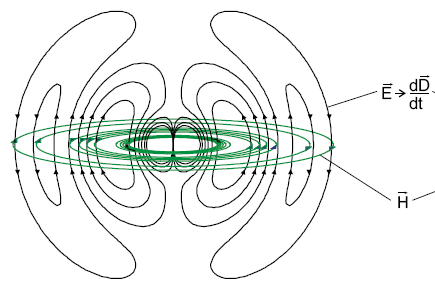
\includegraphics[width=\textwidth]{Abbildungen/Kapitel2/Hertz'scher_Dipol_A.png}
        \caption{}\label{subfig:2_Hertzscher_Dipol_A}
    \end{subfigure}
    \hspace{1cm}
    \begin{subfigure}[c]{0.4\textwidth}
        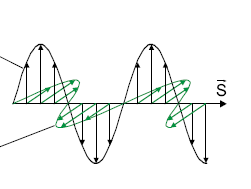
\includegraphics[width=\textwidth]{Abbildungen/Kapitel2/Hertz'scher_Dipol_B.png}
        \caption{}\label{subfig:2_Hertzscher_Dipol_B}
    \end{subfigure}
    \caption{Schematische Darstellung eines Hertz'schen Dipoles mit den umgebenden geschlossenen Wirbelfeldlinien in einer Momentdarstellung nach Quelle~\cite{EM_Schirmung}. Die dargestellte ebene Welle (b) bildet sich in ausreichend großer Entfernung von der Quelle aus.}
    \label{fig:2_Hertzscher_Dipol}
\end{figure}


\subsection{Feldverlauf in der Umgebung eines Dipols}\label{cha:2_sub_Feldverlauf_in_Umgebung_eines_Dipols}

Um die Charakteristik des umgebenden Feldes eines Dipols zu bestimmen ist es zielführend, die Komponenten der Feldstärken in Abhängigkeit des Abstandes zu betrachten. Da die Strahlungsfelder jeder Antenne endlicher Abmessung spärische Wellen sind \cite{Antenna_Theory}, ist weiterhin eine Betrachtung in Kugelkoordinaten $\left(r, \phi, \theta\right)$ zweckmäßig (siehe \Abb \ref{fig:2_Feldverlauf}). 

\begin{figure}
    \centering
    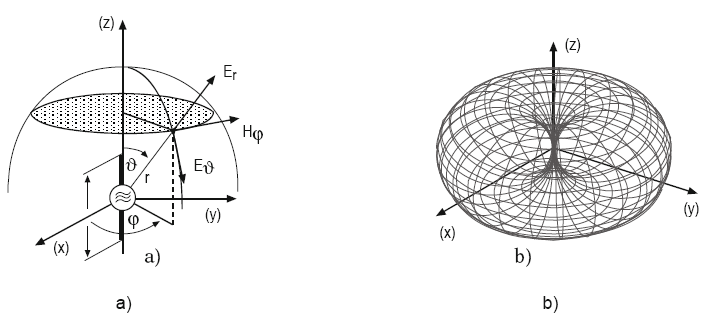
\includegraphics[width=.8\textwidth]{Abbildungen/Kapitel2/Feldverlauf.png}
    \caption[Darstellung der Feldvektoren eines Hertz'schen Dipoles und idealisierter Feldverlauf nach Quelle~\cite{EM_Schirmung}]{Darstellung der Feldvektoren eines Hertz'schen Dipoles in Kugelkoordinaten und idealisierte Darstellung der Feldumgebung ausgehend vom Ursprung nach Quelle~\cite{EM_Schirmung}}
    \label{fig:2_Feldverlauf}
\end{figure}

Für die Amplituden der Feldvektoren, die im Allgemeinen komplex sind, lassen sich demnach folgende Ausdrücke bestimmen \cite{Antenna_Theory}, \cite{EMV}.

\begin{subequations}
\label{eq:2_elektrische_Feldvektoren}
    \begin{align}
        E_r &= \frac{\hat i l \sqrt{\frac{\mu_0}{\varepsilon_0}} \lambda \cos{\theta}}{j 4 \pi^2 r^3}\left(1+ j\frac{2\pi}{\lambda}r\right)e^{-j\frac{2\pi}{\lambda}r} \label{subeq:2_E-Feld1} \\
        E_\phi &= 0 \label{subeq:2_E-Feld2} \\
        E_{\theta} &= \frac{\hat i l \sqrt{\frac{\mu_0}{\varepsilon_0}} \lambda \sin{\theta}}{j 8 \pi^2 r^3}\left(1+ j\frac{2\pi}{\lambda}r + \left(j\frac{2\pi}{\lambda}r\right)^2\right)e^{-j\frac{2\pi}{\lambda}r} \label{subeq:2_E-Feld3}
    \end{align}
\end{subequations}

\begin{subequations}
\label{eq:2_magnetische_Feldvektoren}
    \begin{align}
        H_r &= 0 \hphantom{\text{DiesIstEinLangesPlatzhalterwort1111111111}} \label{subeq:2_H-Feld1}\\
        H_{\phi} &= \frac{\hat i l \sin{\theta}}{4 \pi r^2}\left(1+j\frac{2\pi}{\lambda}r\right)e^{-j\frac{2\pi}{\lambda}r} \label{subeq:2_H-Feld2}\\
        H_{\theta} &= 0
    \end{align}
\end{subequations}

Die \Gleichungen \eqref{eq:2_elektrische_Feldvektoren},~\eqref{eq:2_magnetische_Feldvektoren} sind im gesamten Gebiet bis auf die Quelle selbst gültig \cite{Antenna_Theory}. Mit ihnen lassen sich Interpretationen bezüglich der Eigenschaften einer Antennenumgebung vornehmen:
\par
\vspace{\linespace}
Bei Abständen $r< \lambda / 2\pi$ beginnen die Terme höherer Ordnung zu dominieren. Diese Umgebung wird als Nahfeld bezeichnet und bei der dort befindlichen Energie handelt es sich hauptsächlich um imaginäre, d.h. gespeicherte Energie \cite{Antenna_Theory}. Das Nahfeld kann nach~\cite{Bundesnetzagentur_Glossar_Nahfeld} weiterhin in reaktives und strahlendes Nahfeld, auch als Übergangsfeld bezeichent, unterteilt werden. Für Antennen beliebiger Bauart kann als Grenze zwischen dem reaktiven und dem strahlenden Nahfeld (Fresnel Region) der Abstand $r=0,62 \sqrt{D^3\lambda}$ angesehen werden, wobei $D$ die größte Ausdehnung der Antenne ist \cite{Antenna_Theory}. Im Nahbereich weist das elektrische Feld die beiden Komponenten $E_r$ und $E_{\theta}$ auf. $E_\theta$ und $H_\phi$ sind um \SI{90}{\degree} gegeneinander phasenverschoben~\cite{EM_Schirmung}. Vereinfacht man die Gleichungen unter Vernachlässigung der Terme niedriger Ordnung weisen diese Ähnlichkeit mit Gleichungen eines statischen Dipols auf, sodass im Nahfeldbereich auch von quasiststischen Feldern gesprochen wird. Je nach Antennenbauform kann das elektrische oder magnetische Feld in diesem Bereich überwiegen~\cite{EMV}. 
\par
\vspace{\linespace}
Unabhängig von der Antennenbauart herrscht in großen Abstand von der Antenne ein elektromagnetisches Wellenfeld, das sogenannte Fernfeld. In der Entfernung $r\gg \lambda / 2\pi$ können in den Gleichungen \eqref{eq:2_elektrische_Feldvektoren},~\eqref{eq:2_magnetische_Feldvektoren} die Terme höherer Ordnung vernachlässigt werden. Dabei wird ersichtlicht, dass die Komponente $E_r$ gegenüber $E_\theta$ von niedrigerer Potenz ist und somit in Näherung ebenfalls vernachlässigt werden kann. Somit sind in diesem Bereich nur $E_\theta$ und $H_\phi$ existent. Die beiden Komponenten des elektrischen und magentischen Feldes sind orthogonal zueinander und bilden Transversalelektromagnetische Wellen (TEM). Die Schwingung beider Feldkomponenten erfolgt gleichphasig, sodass das Verhältnis beider Größen im Raum und zeitlich konstant bleibt \cite{EMV}

\begin{equation}
    \frac{E_{\theta}}{H_{\phi}} = Z_0 = \sqrt{\frac{\mu_0}{\varepsilon_0}} = \pi \cdot \SI{120}{\ohm} \approx \SI{377}{\ohm}
\end{equation}

Der Widerstand $Z_0$ wird auch als Feldwellenwiderstand des freien Raumes bezeichnet und ist nur abhängig vom umgebenden Medium~\cite{EMV}. Der Wellenwiderstand $Z$ kann auch formal im Nahfeldbereich aus den Feldvektoren gebildet werden und ist im Allgemeinen eine komplexe Größe.
\par
\vspace{\linespace}
Während der Feldwellenwiderstand, über den die elektrischen und magnetischen Felder miteinander gekoppelt sind, unabhängig der verwendeten Antenne im Fernfeld konstant ist, unterscheiden sich die Verhältnisse der Feldstärken im Nahfeld in Abhängigkeit der Antennenbauart. Hochohmige Nahfelder, welche zum Beispiel Stabantennen umgeben, sind überwiegend elektrischer Natur, während niederohmige Felder von bspw. Rahmenantennen im Vergleich höhere magnetische Feldstärken im Nahfeldbereich aufweisen. In Abhängigkeit des Abstandes zu den Antennen fällt bzw. steigt der Betrags des Feldwellenwiderstandes und nähert sich dem Feldwellenwiderstand des freien Raumes $Z_0$ (siehe \Abb \ref{fig:2_Feldwellenwiderstand}). Für beliebige Antennen wird oft der Abstand $r\geq 2 D^2 / \lambda$ als obere Grenze für das strahlende Nahfeld und damit für den Beginn des Fernfeldes (Fraunhofer Region) genutzt~\cite{Antenna_Theory}.  


\begin{figure}[ht]
    \centering
    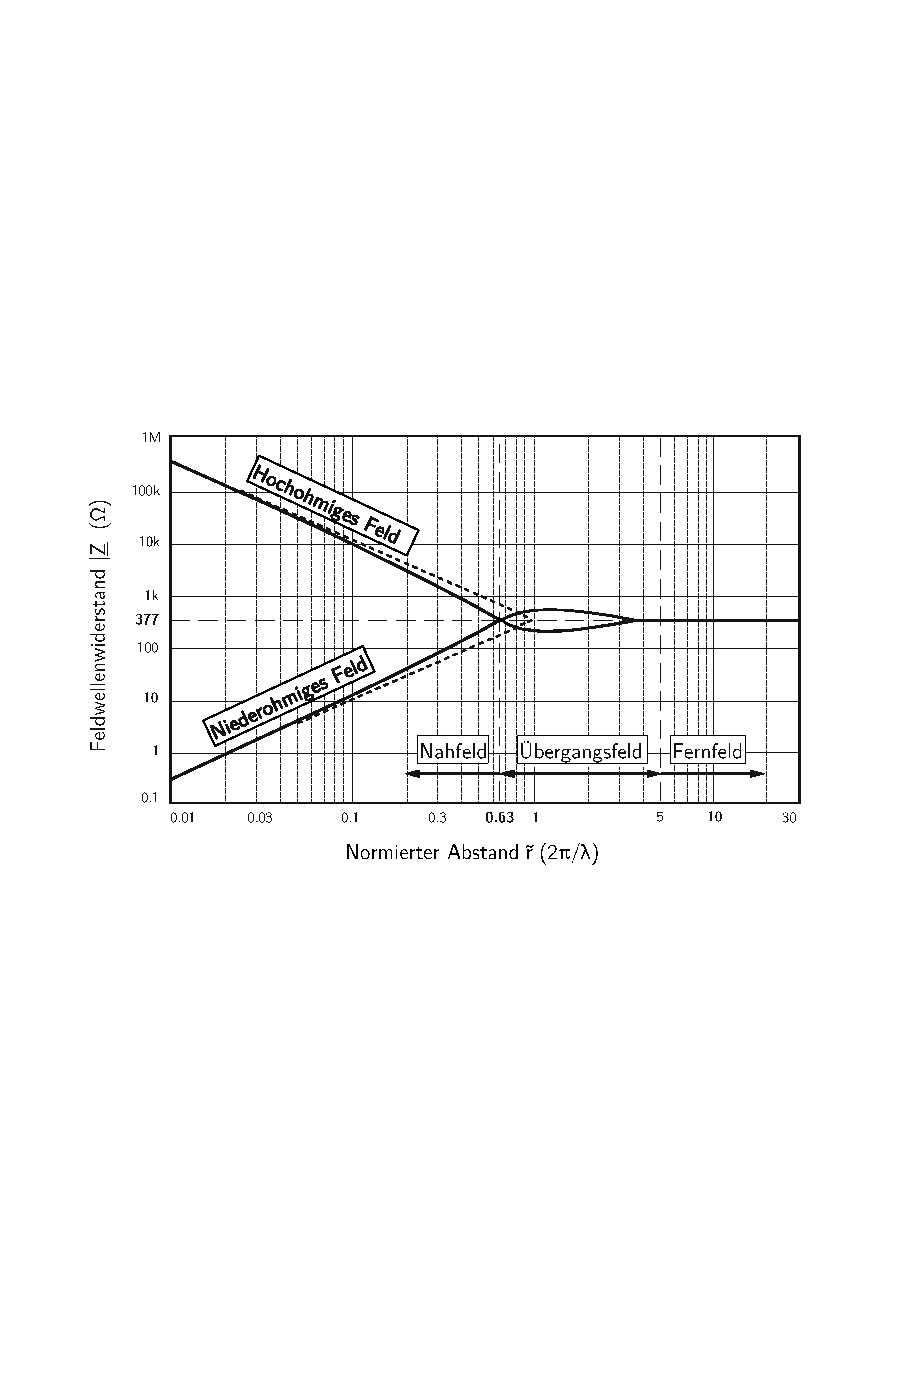
\includegraphics[page=1, width=0.8\textwidth, trim = 1.3cm 8.5cm 1.5cm 7cm, clip]{Abbildungen/Kapitel2/Feldwellenwiderstand.pdf}
    \caption{Verläufe des Feldwellenwiderstandes hoch- und niederohmiger Felder von Stab- und Rahmenantennen in Abhängigkeit des normierten Abstandes von der Feldquelle nach Quelle:~\cite{EMV}}
    \label{fig:2_Feldwellenwiderstand}
\end{figure}


Abhängig von der Art des vorliegenden Feldes unterscheiden sich die Maßnahmen zur Dämpfung und Schirmung maßgeblich voneinander, worauf in den folgenden Abschnitten näher eingegangen wird. Die Abhängigkeit der Natur des vorliegendes Feld, d.h. ist das Feld vorwiegend elektrisch oder magnetisch, in der Nähe einer Antenne von ihrer Bauform ist ebenfalls für Messungen relevant. Für niederfrequente Wechselfelder muss zwischen der Messung elektrischer Felder mit Stabantennen und magnetischer Felder mit Rahmenantennen unterschieden werden. Ab etwa \SI{30}{\mega\hertz} ist die Natur des zu vermessenden Feldes unerheblich für die Bauart der Messantenne, da sich bereits nach kurzem Abstand von der Quelle ein ebenes Wellenfeld ausbildet~\cite{Design_of_shielded_enclosures}.



\subsection{Dämpfung und Absorption}\label{cha:2_sub_Daempfung_und_Absorption}
In verlustbehafteten Medien tritt generell eine Dämpfung der elektrischen und magnetischen Feldstärke einer sich im Medium ausbreitenden Welle auf. Absorption bezeichnet eine sehr starke Dämpfung, wobei die Energie der Welle fast vollständig in Wärme umgesetzt wird. Bei einer von der Frequenz abhängigen Dämpfung wird außerdem die Form der Welle verändert, was als Dispersion bezeichent wird. 
\par
\vspace{\linespace}
Bei der Herleitung der Wellengleichung in Medien endlicher Leitfähigkeit $\sigma > 0$ (siehe \Anhang \ref{Anhang:Herleitung_Wellengleichung}) kann als Abkürzung der Darstellung die komplexe Wellenzahl $k$

\begin{equation}
    k = \sqrt{\varepsilon \mu \omega^2 - j \omega \sigma \mu}
\end{equation}

eingeführt werden. Je größer der Imaginärteil von k, desto größer wird auch die Phasenverschiebung zwischen den elektrischen und magnetischen Feldgrößen~\cite{EM_Schirmung}. Daher bietet sich eine Zerlegung in Real- und Imaginärteil von k an

\begin{equation}
    k = \beta - j \alpha \quad \Leftrightarrow \quad jk = \alpha + j\beta \; ,
\end{equation}

wodurch man die Dämpfungskonstante $\alpha$ und die Phasenkosntante $\beta$ erhält. Diese können wiederum aus $k$ zu

\begin{align}
    \alpha &= \omega \sqrt{\frac{\varepsilon \mu}{2}} \sqrt{\sqrt{1+\left(\frac{\sigma}{\omega\varepsilon}\right)^2}-1} \\
    \beta &= \omega \sqrt{\frac{\varepsilon \mu}{2}} \sqrt{\sqrt{1+\left(\frac{\sigma}{\omega\varepsilon}\right)^2}+1}
\end{align}

bestimmt werden. Mit diesen Koeffizienten kann eine Interpretation der gewünschten Materialeigenschaften für Dämpfungselemente erfolgen. 
\par
\vspace{\linespace}
Für eine möglichst hohe Dämpfung muss $\alpha$ maximal werden. Dies kann durch eine hohe Leitfähigkeit $\sigma$ und hohe Permeabilität $\mu$ erreicht werden. Die Herausforderung ergibt sich jedoch dadurch, dass sich bei großer Änderung der Leitfähigkeit an einer Grenzfläche die Ausbreitungsbedingungen ggf. so stark ändern, dass die Welle nicht gedämpft, sondern reflektiert wird. Für Absorberelemente ist dies jedoch nicht gewünscht, sodass dort eine Dämpfung vor allem durch die Permeabilität erfolgt. Je nach Bauart und Einsatzfrequenz wird dabei dem Magnetfeld Energie durch Ummagnetisierung des Absorbers entzogen, wie es bei Ferritelementen der Fall ist, oder es wird aufgrund der Bauform und mäßiger Leitfähigkeit ein geringer Impdanzsprung hervorgerufen. Letzteres mit mit sogenannten Pyramidenabsorbern erreicht, die aus häufig graphitgetränktem \ac{PU} bestehen und damit ebenfall hochpermeabel sind~\cite{EM_Schirmung}. Je nach Frequenzbereich ist dabei die Höhe der Pyramidenelemente und damit der Winkel der Seitenflächen entscheident für die Absorptionswirkung bei möglichst geringer Reflektion. Je nach Einsatzzweck gibt es ebenfalls unterschiedliche Kombinationen auf Ferrit- und Pyramidenabsorbern, sowie andere Bauformen für spezielle Anwendungen~\cite{EMV-Support_Produktseite}, \cite{Telemeter_Produktseite}. Bei jeglicher Kombination mehrerer Absorber in Reihe entlang der Ausbreitungsrichtung der zu dämpfenden Welle muss wiederum darauf geachtet werden, dass die Leitfähigkeiten an der Grenzfläche möglichst genau übereinstimmen, um keinen Impedanzsprung hervorzurufen, der daraufhin im Sinne der Wellenausbreitung zu einer Grenzschicht führt, die ungewollte Reflektionen hervorruft. Diese Anpassung kann bei Pyramidenabsorbern bspw. durch den Anteil des Kohlenstoffs im Material geschehen~\cite{EM_Schirmung}.




\subsection{Reflektion}\label{cha:2_sub_Reflektion}


Für die Ausbreitung von Wellen im Raum müssen natürlich die im \Abschnitt \ref{cha:2_sub_Verhalten_an_Grenzflächen} vorgestellten Grenzflächen von Materialien einen erheblichen Einfluss haben. Da an der Grenzfläche die Bedingungen für die Feldvektoren \Gleichungen \eqref{eq:2_Flussdichtennormale} eingehalten werden müssen, muss zu einer durchgelassenen Teilwelle (Index \glqq$d$\grqq) stets eine reflektierte Teilwelle (Index \glqq$r$\grqq) hinzukommen, welche Bestandteil der Wellengleichung ist~\cite{EM_Schirmung}.
\par
\vspace{\linespace}
Für den Grenzfall einer idealleitenden Fläche, auf die eine ebene Wellen trifft, muss zum Beispiel die Tangentialkomponente der elektrischen Feldstärke verschwinden~\cite{EM_Schirmung}, was nach \Gleichung \eqref{subeq:2_Feldstaerketangentiale1} zu dem Schluss führt, dass auch die Tangentiale der einfallenden Welle verschwinden muss. Dies kann nur geschehen, indem sich beide gegenseitig vollständig auslöschen, was wiederrum nur bei vollständiger Reflektion geschehen kann.
\par
\vspace{\linespace}
Für eine detailliertere Betrachtung lassen sich zwei Fälle unterscheiden. Im Fall \uproman{1} ist das elektrische Feld parallel zur Einfallsebene, während es im Fall \uproman{2} senkrecht dazu steht (siehe \Abb \ref{fig:2_Wellenreflektion}). In der Darstellung ist die Zeichenebene die Einfallsebene. Da für die Betrachtung von TEM-Wellen und die Relektion an metallischen Oberflächen der Fall \uproman{2} relevant ist, soll hier nur dieser betrachtet werden~\cite{EM_Schirmung}.

\begin{figure}
    \centering
    \begin{subfigure}[c]{0.3\textwidth}
        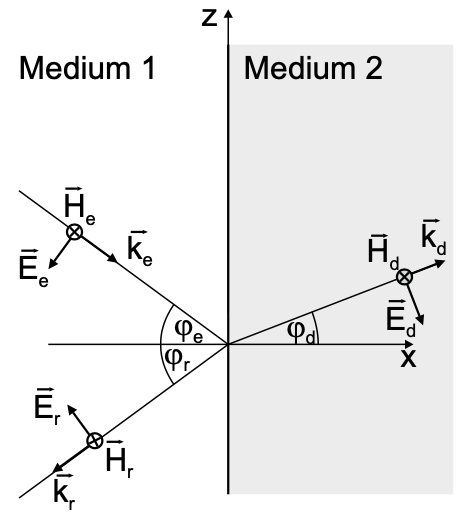
\includegraphics[width=\textwidth]{Abbildungen/Kapitel2/Wellenreflektion_Fall1.png}
        \caption{Fall \uproman{1}\label{subfig:2_Wellenreflektion_Fall1}}
    \end{subfigure}
    \hspace{0.2cm}
    \begin{subfigure}[c]{0.3\textwidth}
        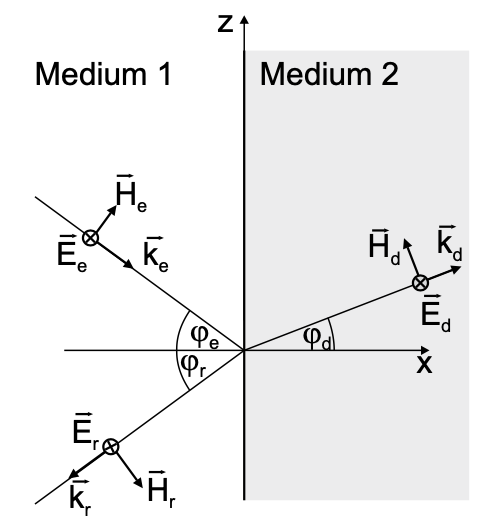
\includegraphics[width=\textwidth]{Abbildungen/Kapitel2/Wellenreflektion_Fall2.png}
        \caption{Fall \uproman{2}\label{subfig:2_Wellenreflektion_Fall2}}
    \end{subfigure}
    \caption[Schematische Darstellung des Auftreffens einer elektromagnetischen Welle auf eine Grenzfläche mit reflektierter und durchgelassener Teilwelle nach Quelle~\cite{EM_Schirmung}]{Schematische Darstellung des Auftreffens einer elektromagnetischen Welle auf eine Grenzfläche mit reflektierter und durchgelassener Teilwelle mit Fallunterscheidung entsprechend der Ausrichtung des elektrischen Feldes zur Einfallsebene (Darstellungsebene) nach Quelle~\cite{EM_Schirmung}.}
    \label{fig:2_Wellenreflektion}
\end{figure}

Für die Feldstärken gelten natürlich die Gleichungen~\eqref{eq:A_Wellengleichungen_mit_Leitfaehigkeit} aus der Herleitung der Wellengleichung im \Anhang \ref{Anhang:Herleitung_Wellengleichung}. Angewandt auf die dargestellten geometrischen Verhältnisse ergibt sich für die einfallende Welle (Index \glqq$e$\grqq)~\cite{EM_Schirmung}

\begin{align}
    \vec E_e &= E_0 e^{-j\vec k_e \vec r} \vec e_y \\
    \vec H_e &= \frac{E_0}{Z_1} \sin{\varphi_e} e^{-j \vec k_e \vec r} \vec e_x + \frac{E_0}{Z_1} \cos{\varphi_e} e^{-j \vec k_e \vec r} \vec e_z \\
    \vec k_e &= k_1 \cos{\varphi_e} \vec e_x - k_1 \sin{\varphi_e} \vec e_z \\
    Z_1 &= \frac{E_0}{H_0}
\end{align}

als Ausgangspunkt für die Betrachtung der Reflektion an einer Grenzfläche. Dabei ist zu berücksichtigen, dass hier die Ausbreitung, im Gegensatz zu \Gleichungen \eqref{eq:A_Wellengleichungen_mit_Leitfaehigkeit}, nicht in Richtung der x-Achse erfolgt, sondern entlang einer beliebigen Richtung. Dafür kann der Ortsvektor $\vec r$ als Ausgangspunkt und der Wellenzahlvektor $\vec k$ als Richtungsvektor mit
$|\vec k| = k = \sqrt{\varepsilon \mu \omega^2 - j \omega \sigma \mu} $ eingeführt werden~\cite{EM_Schirmung}. \par \vspace{\linespace} Analog kann für die reflektierte und die durchgelassene Teilwelle mit dem Reflektionsfaktor $R_{\uproman{2}}$ und dem Durchlassfaktor $D_{\uproman{2}}$

\begin{align}
    E_r &= E_0 R_{\uproman{2}} e^{-j\vec k_r \vec r} \vec e_y \\
    \vec H_r &= \frac{E_0}{Z_1} R_{\uproman{2}} \sin{\varphi_r} e^{-j \vec k_r \vec r} \vec e_x - \frac{E_0}{Z_1} R_{\uproman{2}} \cos{\varphi_r} e^{-j \vec k_r \vec r} \vec e_z \\
    \vec k_e &= - k_1 \cos{\varphi_r} \vec e_x - k_1 \sin{\varphi_r} \vec e_z \\
    E_d &= E_0 D_{\uproman{2}} e^{-j\vec k_d \vec r} \vec e_y \\
    \vec H_d &= \frac{E_0}{Z_2} D_{\uproman{2}} \sin{\varphi_d} e^{-j \vec k_d \vec r} \vec e_x + \frac{E_0}{Z_2} D_{\uproman{2}} \cos{\varphi_d} e^{-j \vec k_d \vec r} \vec e_z \\
    \vec k_d &= k_1 \cos{\varphi_d} \vec e_x - k_1 \sin{\varphi_d} \vec e_z
\end{align}

geschrieben werden. Unter Zuhilfenahme der Gesetzmäßigkeiten an Grenzflächen \Gleichungen \eqref{eq:2_Feldstaerketangentiale} für die Stelle $x=0$ lassen sich folgende Ausdrücke für den Reflektions- und den Durchlassfaktor finden, die das Verhältnis der beiden Teilwellen nach Auftreffen auf eine Grenzschicht beschreiben:

\begin{align}
    R_{\uproman{2}} &= \frac{Z_2 \cos{\varphi_e} - Z_1 \cos{\varphi_d}}{Z_2 \cos{\varphi_e} + Z_1 \cos{\varphi_d}} \\
    D_{\uproman{2}} &= \frac{2 Z_2 \cos{\varphi_e}}{Z_2 \cos{\varphi_e} + Z_1 \cos{\varphi_d}} \\ 
    1 &= D_{\uproman{2}} - R_{\uproman{2}} = D_{\uproman{2}} \frac{Z_1 \cos{\varphi_d}}{Z_2 \cos{\varphi_e}} + R_{\uproman{2}} \; .
\end{align}

Für den Fall, dass an der Grenzfläche kein Materialübergang stattfindet ($Z_1 = Z_2$), gilt $\varphi_e = \varphi_d$ und damit $R_{\uproman{2}} = 0$ und $D_{\uproman{2}} = 1$, das bedeutet die Welle wird nicht gebeugt und es findet keine Reflektions statt. Handelt es sich bei Medium 2 dagegen um einen idealen Leiter mit $Z_2 = 0 \neq Z_1$, so wird $D_{\uproman{2}} = 0$ und $R_{\uproman{2}} = -1$, was entsprechent der Erwartung heißt, dass eine eintreffende Welle an einer idealisierten metallischen Oberfläche vollständig reflektiert wird~\cite{EM_Schirmung}. 









\section{Theorie der elektromagnetischen Schirmung}\label{cha:2_Theorie_der_elektromagnetischen_Schirmung}

Wie bereits im vorherigen \Abschnitt \ref{cha:2_Wellenausbreitung} angedeutet, besitzen elektromagnetische Felder in Abhängigkeit ihrer Frequenz unterschiedliche Eigenschaften, welche unterschiedliche Schirmungsmechanismen in Bezug auf die Abmessung der verwendeten Anordnung und der Art des Feldes notwendig machen. Da die Messungen im Rahmen dieser Arbeit im Fernfeld einer Antenne stattfinden sollen und auch der zu nutzende Freqeunzbereich mit $1\ldots$\SI{18}{\giga\hertz} deutlich über der Grenze von \SI{30}{\mega\hertz} liegt, ab der man nach~\cite{Design_of_shielded_enclosures} von der Ausbreitung ebener Wellen unabhängig von der Antennenbauart ausgegehen kann, soll sich die Betrachtung von Schirmungsmethoden auf das sogenannte elektromagnetische Wellenfeld beschränkten. Dies deckt sich mit der Einteilung elektromagnetischer Felder nach~\cite{Feldtheorie_Begriffe} und dem Richtwert für die Anwendung der Schirmungsmechanismen für Wellenfelder nach~\cite{EM_Schirmung}

\begin{equation}
    f > \frac{c_0}{d}
\end{equation}

mit einer Schirmabmessung $d$ im Bereich von \SI{1}{\meter} und Frequenzen $f$ im Bereich von $1\ldots$\SI{18}{\giga\hertz}.

%Induktion als charakteristisches Merkmal in diesem Anwednungsbreich



\subsection{Begriffe der Schirmdämpfung}\label{cha:2_sub_Begriff_der_Schirmdaempfung}

Um im Weiteren eine einheitliche Begriffsgrundlage vorauszusetzen, soll an dieser Stelle kurz auf die relevanten Begriffe der elektromagnetischen Strahlung und Schirmung eingegangen werden. Außerdem soll unter anderem die im Folgenden angewandte Konvention zur Darstellung von Bezugsgrößen logarithmierter Verhältnisse von Größen kurz eingeführt werden. 

\subsubsection{Pegelmaße}

Generell wird für die Darstellung von Verhältnissen elektrischer und magentischer Feldgrößen gern auf logarithmische Verhältnisse, sogenannte Pegel in Dezibel zurückgegriffen, was nicht nur den Vorteil eines großen Dynamikbereiches in der Darstellung hat, sondern auch verschiedene Rechnungen erleichtert. Unterschieden wird dabei zwischen relativen und bezogenen Pegeln. Relative Pegel, auch als Übertragungsmaße bezeichnet, stellen die Verhältnisse zweier Größen dar und dienen damit der Charakterisierung von Dämpfungen oder dem Ausdruck von Antennengewinnen. Für Feldgrößen $X$, wie Spannung, Ströme oder Feldstärken, ist der relative Pegel anders definiert~\cite{EM_Schirmung}

\begin{equation}
    X \; \left[\si{\Dezibel}\right] = 20 \cdot \log_{10} \left( \frac{X_1}{X_2} \right) = 20 \cdot \lg \left( \frac{X_1}{X_2} \right)
\end{equation}

als für Leistungen $P$

\begin{equation}
    p \; \left[\si{\Dezibel}\right] = 10 \cdot \lg \left( \frac{P_1}{P_2} \right) \; .
\end{equation}

Dies hat den Vorteil, dass bei der Rechnung mit Pegeln nicht auf die Art des vorliegenden Verhältnisses geachtet werden muss. Für ein intuitiveres Verständnis der Bedeutung bestimmter Pegel für das reale Großenverhältnis zweier Feldgrößen bzw. Leistungen sind in der \Tabelle\ref{tab:2_Relative_Pegel} gängige Pegel beispielhaft dargestellt.

\begin{table}
\renewcommand{\arraystretch}{\tablestretch}
\centering
\caption{Verschiedene relative Pegel mit zugehörigen Verhältnissen von Feldgrößen und Leistungen}
\vspace{\tablespace}
\begin{tabular}{l c c}
    \toprule
    Relativer Pegel $\left[\si{\Dezibel}\right]$ & Verhältnis von Feldgrößen & Verhältnis von Leistungen \\
    \midrule
    3   &   1,412   &   1,995   \\
    6   &   1,995   &   3,981   \\
    10  &   3,162   &   10      \\
    40  &   100     &   10.000  \\
    60  &   1000    &   1.000.000 \\
    80  &   10.000  &   $10^8$  \\
    100 &   100.000  &   $10^{10}$ \\
    \bottomrule
\end{tabular}
\label{tab:2_Relative_Pegel}
\end{table}

Bezogene Pegel beschreiben im Gegensatz dazu Absolutwerte einer Größe in Bezug auf einen Referenzwert, beispielsweise einen ungestörten Raumpunkt. Um wieder auf den ursprünglichen Wert der Größe schließen zu können, ist eine Angabe der Bezuggröße notwendig. Diese soll nach~\cite{IEC60027-3} wie folgt erfolgen: 

\begin{equation}
    p_{1 \si{\milli\watt}} = 10 \cdot \lg \left( \frac{P_1}{1 \si{\milli\watt}}\right) \si{\Dezibel} \; .
\end{equation}

Auf eine Kennzeichnung des Bezuges an der Einheit $\si{\Dezibel}$ soll ausdrücklich verzichtet werden, obwohl dies in der Literatur die vorherrschende Schreibweise ist. Für diese Arbeit soll jedoch die nach~\cite{IEC60027-3} korrekte Schreibweise $p_{1 \si{\milli\watt}} = 3 \si{\Dezibel}$ angewandt werden. 


\subsubsection{Schirmdämpfung}\label{cha:2_subsub_Schirmdaempfung}

Ein Schirm wird im Allgemeinen im Rahmen elektromagnetischer Anwendung dazu eingesetzt, Feldstärken im einem bestimmten Bereich innerhalb oder außerhalb des Schirms zu dämpfen. Nach dem Reziprozitätsgesetz ist es bei gleicher Feldverteilung, auch wenn diese in der Praxis oft nur bedingt gegeben ist~\cite{EMV-gerechtes_Geraetedesign}, dabei unerheblich, ob sich die Quelle des Feldes innerhalb oder außerhalb der Schirmgrenzen befindet~\cite{EM_Schirmung}. Die Schirmwirkung lässt sich mit dem Schirmfaktor $Q$, der die Feldstärke an einem Raumpunkt nach der Anwendung des Schirms (Index \glqq$1$\grqq) zur Feldstärke ohne Schirm (Index \glqq$0$\grqq) in Verhältnis setzt

\begin{align}
    Q_e = \frac{E_1}{E_0} \; \text{,}
\end{align}

beurteilen~\cite{EM_Schirmung}.
\par
\vspace{\linespace}
Die im Allgemeinen verursachte Phasenverschiebung durch den Schirm, macht $Q$ zu einer komplexen Größe~\cite{EM_Schirmung}. Da in den meisten Fällen jedoch vor allem der Betrag von Interesse ist, wird die Schirmdämpfung $a_S$ als Pegelmaß der Feldgrößenbeträge definiert:

\begin{align}
    a_e &= 20 \cdot \lg \left(\frac{\abs{E_0}}{\abs{E_1}}\right) = 20 \cdot \lg \frac{1}{\abs{Q_e}} \\
    a_m &= 20 \cdot \lg \left(\frac{\abs{H_0}}{\abs{H_1}}\right) = 20 \cdot \lg \frac{1}{\abs{Q_m}} \\
    a_S &= 10 \cdot \lg \left(\frac{\abs{P_0}}{\abs{P_1}}\right) \; \text{.}
\end{align}

Die Schirmdämpfung in Dezibel wird für ausgedehnte Schirme, aufgrund der teilweise starken Schwankungen zwischen einzelnen Raumpunkten hinsichtlich Feldverteilung und Frequenzen, nur als minimal erreichte Schirmdämpfung angegeben, da nur dieser Wert bspw. zur Charakterisierung der Schirmwirkung eines Gehäuses sinnvoll ist~\cite{EM_Schirmung}. Da nach der Definition der Schirmdämpfung die Feldgrößen einmal mit und einmal in Abwesenheit eines Schirmes gemessen werden muss und dies nicht zeitgleich erfolgen kann, bezeichnet man die Bestimmung der Schirmwirkung auch als Einfügungsmessung, da der Schirm im Verlauf der Messung zwischen Sende- und Empfangseinrichtung eingefügt wird. Auf die unterschiedlichen Messmethoden wird im \Abschnitt\ref{cha:2_Methoden_der_Schirmdaempfungsmessung} genauer eingegangen.


\subsection{Schirmung ebener Wellenfelder}\label{cha:2_sub_Schirmung_ebener_Wellenfelder}

Generell kann die Aussage getroffen werden, dass sich magnetostatische Gleichfelder von allen Feldarten am allerschwersten und nur mit hohen konstruktiven Aufwand abschirmen lassen~\cite{EM_Schirmung}. Vorteilhaft bei der Schirmung von Wellenfeldern ist im Gegensatz dazu die vorliegende Veränderung der magnetischen Feldstärke, welche elektrische Felder im Schirmmaterial induzieren können~\cite{Maxwell}


\begin{equation}
    \text{rot} \; \vec E= - \frac{\partial \vec B}{\partial t} \; \text{.}
    \label{eq:2_Induktionsgesetz}
\end{equation}

Mithilfe des Durchflutungsgesetzes~\cite{Maxwell}

\begin{equation}
    \text{rot} \; \vec H = \vec j_L + \frac{\partial \vec D}{\partial t}
    \label{eq:2_Durchflutungsgesetz}
\end{equation}

kann dies zur Schaffung eines wirksamen Schirmes genutzt werden. Für Frequenzen oberhalb von \SI{30}{\mega\hertz} und Feldquellen mit mehr als wenigen Zentimeter Abstand zum Schirm muss die Schirmdämpfung deshalb nicht für magnetische und elektrische Felder gesondert berechnet werden~\cite{Design_of_shielded_enclosures}. Dies gilt insbesondere für die Absorbtionsverluste im Material (siehe \Abschnitt\nameref{cha:2_subsub_Schirmungseffektivitaet}), die unabhängig vom Typ der Feldquelle sind~\cite{NASA_SP-3067}.   
\par 
\vspace{\linespace}
Die Wirkungsweise wird bei Betrachtung eines leitfähigen Materialblockes schnell deutlich. Bei Durchsetzung mit einem statischen Magnetfeld durchdringt dieses den Block vollständig und ohne jegliche Schirmung unter der Annahme $\mu = 1$. Handelt es sich bei dem Magnetfeld nun allerdings um ein Wechselfeld mit $f > 0$, so wird nach \Gleichung\eqref{eq:2_Induktionsgesetz} ein elektrisches Wirbelfeld um die magnetischen Flusslinien induziert~\cite{EM_Schirmung}. Im leitfähigen Material bilden sich daraufhin Wirbelströme aus, die nach \Gleichung\eqref{eq:2_Durchflutungsgesetz} ihrerseits ein Magnetfeld erzeugen, dass nach der Lenz'schen Regel seiner Ursache, also dem ursprünglichen, äußeren Magnetfeld entgegengerichtet ist und dieses durch Überlagerung abschwächt~\cite{EM_Schirmung}. Mit höherer Frequenz des Magnetfeldes und höherer Leitfähigkeit des Schirms steigt die Schirmwirkung des Materials aufgrund der besser fließenden Wirbelströme. Je höher die Frequenz, umso stärker verdichten sich die Magnetfeldlinien des äußeren und des Gegenfeldes am Rand des Materials, ebenso wie die Stromdichte~\cite{EM_Schirmung}. Dieser als Stromverdrängung bekannte Effekt führt bei hoher Frequenz dazu, dass die induzierten Ströme nur noch auf der äußeren Randschicht des Schirmmaterials fließen, was ebenfalls als Skineffekt bekannt ist. In diesem Falls wirkt nur die äußere Materialschicht dem anliegenden Feld entgegen, sodass die gleiche Schirmwirkung mit einer hohlen, leitfähigen Hülle erreicht werden kann, welche damit auch die einfachste Möglichkeit eines elektrodynamischen Schirmes darstellt. 
\par 
\vspace{\linespace}
Die vorausgesetzte hohe Leitfähigkeit des Schirms hat außerdem den Vorteil, auch als Faraday'scher Käfig zu wirken und in hohem Maße elektrische Gleich- und Wechselfelder zu schirmen. Die erreichte Güte bei der Schirmung elektrischer Felder ist dabei bei gleichem Aufwand um Größenordnungen höher als die spezieller dielektrischer Schirme~\cite{EM_Schirmung}.
\par
\vspace{\linespace}
Für die beschriebene Wirkungsweise der Schirmung ist weiterhin unerheblich, ob es sich bei dem Störfeld um ein quasitatisches oder ein ebenes Wellenfeld handelt~\cite{EM_Schirmung}. Ein Faraday'scher Käfig ist damit die effektivste Methode zur Schirmung elektrodynamischer Felder. Für Wellenfelder, deren Abmessung in der Größenordnung der Schirmausdehnung liegt, müssen jedoch Besonderheiten berücksichtigt werden, auf die im \Abschnitt\nameref{cha:2_subsub_Hohlraumresonanzen} eingegangen wird.  


\subsubsection{Eindringtiefe}\label{cha:2_subsub_Eindringtiefe}

Wie bereits beschrieben sind für die Eindringtiefe $\delta$, oder auch äuivalente Leitschichtdicke genannt, der Felder in des Schirmmaterial nicht nur die Materialparameter wie Leitfähigkeit $\sigma$ und Permeabilität $\mu$ entscheident, sondern auch die Frequenz des äußeren Feldes. Der Wert der Eindringtiefe ist für die vorliegende Situation nach~\cite{Taschenbuch_HF-Technik} definiert als

\begin{equation}
    \delta = \sqrt{\frac{1}{\pi f \mu \sigma}}
    \label{eq:2_Eindringtiefe}
\end{equation}

und gibt an, in welcher Entfernung von der Randschicht ein äußeres Feld um den Faktor $1/e \approx 37 \si{\percent}$ abgeschwächt wird~\cite{Taschenbuch_HF-Technik}. Innerhalb des Schirmmaterials entspricht der Feldverlauf dem einer gedämpften Welle~\cite{EM_Schirmung}. Für die richtige Dimensionierung eines elektrodynamischen Schirmes spielt die Eindringtiefe also eine wichtige Rolle, ebenso für eine geeignete Materialauswahl.


\subsubsection{Schirmungseffektivität}\label{cha:2_subsub_Schirmungseffektivitaet}

Für die Bestimmung der Effektivität eines Schirmes gegen eindrigende Strahlung ist jedoch nicht nur der Absorbtionsverlust durch Erzeugung von Wirbelfeldern, sondern auch der reflektierte Anteil der eintreffenden Welle (vergleiche \Abschnitt\ref{cha:2_sub_Reflektion}) entscheident. Nach~\cite{Problems_in_shielding_electronic_equiptment, NASA_SP-3067} ergibt sich die Schirmungseffektivität $S$ in Dezibel aus

\begin{equation}
    S_w \; \left[\text{dB}\right] = R_w \; \left[\text{dB}\right] + A_w \; \left[\text{dB}\right] + B_w \; \left[\text{dB}\right]
\end{equation}

mit dem Reflektionsverlust \acs{R_w}, der Absorbptionsdämpfung \acs{A_w} und dem Korrekturfaktor \acs{B_w} für Reflektionen innerhalb des Schirms bzw. beim Übergang der inneren Grenzflächen (vgl. \Abschnitt\ref{cha:2_sub_Verhalten_an_Grenzflächen}). Für $A_w > 15 \si{\Dezibel}$ kann \acs{B_w} jedoch vernachlässigt werden~\cite{NASA_SP-3067}. In dem Fall, dass die Feldquelle mehr als eine Wellenlänge $\lambda$ oder in einem Abstand von mindestens $D^2 / \lambda$, mit der größten Ausdehnung der Feldquelle $D$, vom Schirm entfernt positioniert ist, ist für die Bestimmung von \acs{R_w} nach~\cite{NASA_SP-3067} die Beziehung für ebene Wellen in jedem Fall ausreichend.  
\par
\vspace{\linespace}
Zur einfacheren Bestimmung der Summanden \acs{R_w} und \acs{A_w} kann auf Nomogramme zurückgegriffen werden. Somit kann für eine gegebene Frequenz der zu schirmenden Welle und ein ausgewähltes Material direkt der entsprechende Verlust beim Materialdurchgang abgelesen werden. Im \Anhang\ref{Anhang:Nomogramm_Reflektionsdaempfung} und \Anhang\ref{Anhang:Nomogramm_Absorptionsverlust} sind die Schaubilder nach~\cite{Simplified_shielding} dargestellt. 
\par
\vspace{\linespace}
Beispielhaft ergeben sich folgende Dämpfungen für \SI{2}{\milli\meter} starke Bleche aus Aluminium und Stahl bei \SI{100}{\mega\hertz} und \SI{10}{\giga\hertz}:


\begin{table}[h]
    \renewcommand{\arraystretch}{\tablestretch}
    \centering
    \caption[Ausgewählte Absorptions-, Reflektionsdämpfungen verschiedener Bleche]{Ausgewählte Absorptions-, Reflektionsdämpfungen verschiedener Bleche (\SI{2}{\milli\meter})}
    \vspace{\tablespace}
    \begin{tabular}{p{2cm} p{3cm} C{2.5cm} C{2.5cm}}
    \toprule
    Frequenz & Material & $R_w \; [\si{\Dezibel}]$ & $A_w \; [\si{\Dezibel}]$  \\
    \midrule
    \SI{100}{\mega\hertz} & Aluminium   &  86 &  >1000 \\
    \SI{10}{\giga\hertz} & Aluminium    &  66 &  >1000 \\
    \SI{100}{\mega\hertz} & Stahl       &  58 &  >1000 \\
    \SI{10}{\giga\hertz} & Stahl        &  38 &  >1000 \\
    \bottomrule
    \end{tabular}
    \label{tab:2_Beispielwerte_Schirmdaempfungen}
\end{table}

Wie leicht zu erkennen ist, nehmen die Absorptionsverluste im Material bei den betrachteten Frequenzen trotz der geringen Materialstärke bereits so hohe Werte an, dass praktisch davon ausgegangen werden kann, dass die Welle im Schirm vollständig ausgelöscht wird. Für Aluminium und andere \ac{NE-Metalle} ist dies durch die hohe Leitfähigkeit zu erklären (vgl. \Gleichung\eqref{eq:2_Eindringtiefe}), bei ferromagnetischen Materialien spielt die Permeabilität zusätzlich eine große Rolle für die Eindringtiefe elektromagnetischer Wellen in einen Schirm und damit die erreichbare Schirmdämpfung bei einer gegebenen Materialstärke. 
\par 
\vspace{\linespace}
Die höheren Reflektionsdämpfungen des Aluminiums sind auf die höhere Leitfähigkeit $\sigma$ im Vergleich zu Stahl zurückzuführen. Auch wenn diese für die Einfügungsdämpfung keinen nennenswerten Beitrag leisten, werden sie bei der Betrachtung von Hohlraumresonanzen innerhalb eines Schirmes relevant. 
\par
\vspace{\linespace}
Die theoretisch erreichbare Schirmdämpfung von mehr als \SI{1000}{\Dezibel} reduziert sich in der Praxis natürlich durch jegliche Öffnungen des Systems, durch die Störungen einkoppeln bzw. nach dem Reziprozitätsgesetz auskoppelt können. Für verschraubte Metallgehäuse kann bei sorgfältiger Platzierung der Verschraubungen eine Dämpfung von >\SI{100}{\Dezibel} erreicht werden~\cite{Design_of_shielded_enclosures}. Mit steigender Frequenz nimmt die praktisch erreichbare Schirmung ebenfalls ab, da die elektromagnetischen Wellen aufgrund der kürzeren Wellenlänge leichter über Spalte in das System gelangen können. Zu beachten ist auch, dass die theoretischen Schirmungseffektivitäten $S_w \geq 150 \si{\Dezibel}$ messtechnisch kaum oder nur mit großem Aufwand nachweisbar sind~\cite{EM_Schirmung}.
\par
\vspace{\linespace}
Zur Vermeidung von nichtlinearen Sättigungserscheinungen des Schirms werden in der Praxis des Weiteren häufig mehrschichtige Schirme eingesetzt, wobei die der Störung zugewandte Seite möglichst aus einem linearen Schirmmaterial mit niedriger Permeabilität bestehen sollte~\cite{EMV}. 



\subsubsection{Hohlwellenleiter}\label{cha:2_subsub_Hohlwellenleiter}
Das Phänomen der vollständigen Reflektion ebener Wellen an idealleitendes Flächen (vgl. \Abschnitt\ref{cha:2_sub_Reflektion}) legt eine Anwendung von Hohlkonstruktionen als Wellenleiter nahe. 
\par
\vspace{\linespace}
\begin{figure}
    \centering
    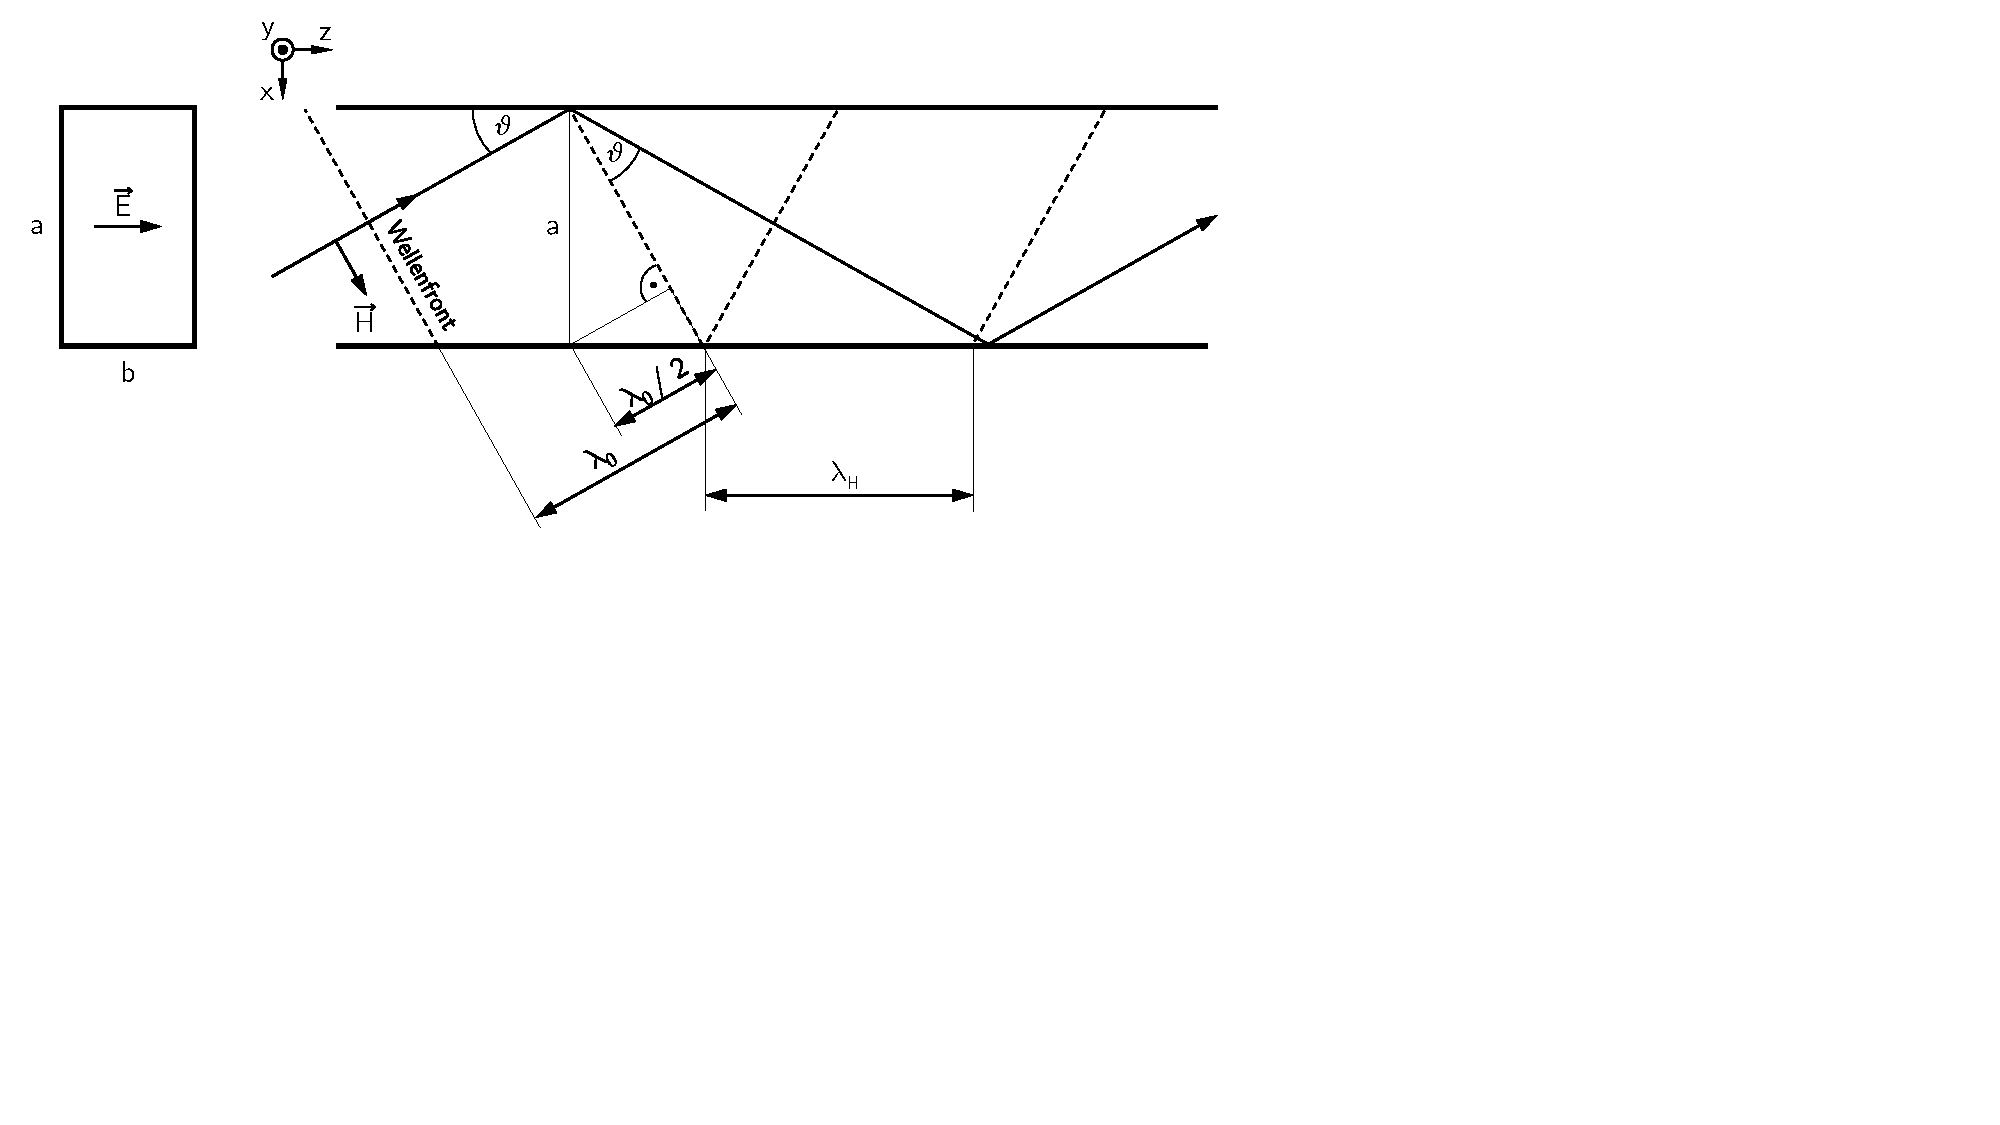
\includegraphics[scale = 1, trim = 0cm 10cm 13cm 0cm, clip, width=.8\textwidth]{Abbildungen/Kapitel2/Hohlwellenleiter.pdf}
    \caption{Schematische Darstellung eines Hohlwellenleiters im Schnitt nach~\cite{Taschenbuch_HF-Technik}}
    \label{fig:2_Hohlwellenleiter}
\end{figure}

Wird für eine ebene Welle, wie in \Abb\ref{fig:2_Hohlwellenleiter} dargestellt, ein E-Feldvektor parallel der Seitenwände mit einem zugehörigen H-Feldvektor angenommen, ist der Winkel $\vartheta$, unter dem die Ausbreitung der Welle stattfindet, nur von der längsten Seite des Hohlwellenleiters $a$ und der Freiraumwellenlänge $\lambda_0$ abhängig~\cite{Taschenbuch_HF-Technik}. Die Ausbreitungsbedingung ergibt sich aus dem Gangunterschied der reflektierten Wellenanteile, die sich möglichst konstruktiv überlagern sollten, d.h. einen Gangunterschied von $\lambda_0 / 2$ aufweisen sollten. Für das dargestellt Beispiel ergibt sich: 

\begin{equation}
    \sin{\vartheta} = \frac{n \cdot \lambda_0}{2 a} \; , \qquad n \in \mathbb{N}
\end{equation}
 
Mit $n=1$ wird dabei die Grundwelle beschrieben und mit $n>1$ die sogenannten höheren Wellentypen~\cite{Taschenbuch_HF-Technik}.
\par
\vspace{\linespace}
Die in  \Abb\ref{fig:2_Hohlwellenleiter} dargestellten gestrichelten Linien stellen die Ebenen konstanter Phase dar und deren Abstand ist die Hohlleiterwellenlänge $\lambda_H$ für die gilt~\cite{Taschenbuch_HF-Technik}:

\begin{equation}
    \lambda_H = \frac{\lambda_0}{\cos{\vartheta}}
\end{equation}

Mit sinkender Frequenz steigt also der Winkel $\vartheta$ und ebenfalls $\lambda_H$, bis für $\vartheta = 90\si{\degree}$ die Hohlleiterwellenlänge gegen unendlich geht. Das bedeutet es gibt eine untere, kritische Frequenz $f_k$, für die keine Wellenausbreitung im Hohlwellenleiter stattfinden kann. Dies kann für Öffnungen und Durchführungen in Schirme genutzt werden.
\par
\vspace{\linespace}
Zur Bestimmung der Grenzfrequenzen in verschiedenen Leiterquerschnitten müssen verschiedene Wellentypen unterschieden werden. H-Wellen (TE-Wellen, transversal-elektrisch) haben nur eine axiale magnetische Komponenten $H_z$ und E-Wellen (TM-Wellen, transversal-magnetisch) nur eine Längskomponente des elektrischen Feldes $E_z$, während die jeweils anderen axialen Komponenten Null sind~\cite{Taschenbuch_HF-Technik}. Die Kennzeichnung der Wellentypen geschieht über Indizes, die die Maxima in den unterschiedlichen Koordinantenrichtungen beschreiben. Die Grundwelle ist dann jeweils der Wellentyp, der innerhalb eines Querschnittes noch ausbreitungsfähig ist~\cite{Taschenbuch_HF-Technik}. In \Tabelle\ref{tab:2_Grenzwellenlaengen_Hohlleiter} sind die kritischen Wellenlängen für verschiedene Querschnitte mit den jeweiligen Grundwellentypen nach~\cite{Taschenbuch_HF-Technik} zusammengefasst.


\begin{table}[ht]
    \centering
    \renewcommand{\arraystretch}{\tablestretch}
    \caption{Kritische Wellenlängen für die Ausbreitung in verschiedenen Querschnitten mit Grundwellenform nach~\cite{Taschenbuch_HF-Technik}}\label{tab:2_Grenzwellenlaengen_Hohlleiter}
    \vspace{\tablespace}
    \begin{threeparttable}
    \begin{tabular}{p{5cm} p{4cm} C{3cm}}
    \toprule
        Hohlleiterquerschnitt & Anregung & $\lambda_k$ \\
    \midrule
        Rechteckquerschnitt & $H_{10}$-Mode & $2a$ \\
        Kreisquerschnitt    & $E_{01}$-Mode & $\approx 1,305 d$ \\
        Kreisquerschnitt    & $H_{11}$-Mode & $\approx 1,705 d$ \\
        Sechseckquerschnitt & $H_{10}$-Mode & $2a $\footnotemark[1] \\
    \bottomrule
    \end{tabular}
    \begin{tablenotes}
    \footnotesize
    \item[1] Näherung nach~\cite{EM_Schirmung} mit dem größten Abstand zweier Seiten $a$
    \end{tablenotes}
    \end{threeparttable}
\end{table}

\par
\vspace{\linespace}
Wellen mit $f < f_k$ erfahren innerhalb eines Hohlleiters mit der Länge $l$ eine Dämpfung~\cite{EM_Schirmung}:

\begin{align}
    S_{WL} \left[\si{\Dezibel}\right] &= 20\log_{10}\left(e^{\alpha\cdot l}\right)  \\
    \alpha &= \frac{2\pi}{\lambda_k} \sqrt{1-\left(\frac{\lambda_k}{\lambda_0}\right)^2} = \frac{2\pi f_k}{c_0} \sqrt{1-\left(\frac{f}{f_k}\right)^2} \qquad \text{für} \quad f < 0,8 f_k
\end{align}




\subsubsection{Hohlraumresonanzen}\label{cha:2_subsub_Hohlraumresonanzen}

Die Betrachtung des vorangegangenen \Abschnitts\nameref{cha:2_subsub_Hohlwellenleiter} kann im Weiteren auf ein geschlossenes, leitfähiges Gehäuse ausgeweitet werden, das im Wesentlichen einen Hohlwellenleiter mit kurzgeschlossenen Enden darstellt. Entsprechend der Grenzbedingungen für das elektrische und magnetische Feld (vgl. \Abschnitte\ref{cha:2_sub_Verhalten_an_Grenzflächen},~\ref{cha:2_sub_Reflektion}) wird eine eingekoppelte Hohlleiterwelle im Idealfall an den Gehäuseenden vollständig reflektiert. Die Überlagerung der hin- und rücklaufenden Welle führt bei ausgezeichneten Anregungsfrequenzen zum Resonanzfall, wodurch ein sogenannter Hohlraumresonator entsteht. Anschaulich ist klar, dass zum Auftreten einer Resonanz eine stehende Welle mit einem ganzzahligen Vielfachen ihrer Wellenlänge in den Bereich der Schirmabmessung kommen muss.
\par
\vspace{\linespace}
Aufgrund der dabei entstehenden hohen Verstärkung der Hohlraumwelle kann im Bereich dieser Frequenzen eine deutliche Reduktion der Schirmwirkung des Gehäuses beobachtet werden~\cite{EM_Schirmung}. Ein gängiger Weg zur Reduktion dieses Phänomens ist der Einsatz von Absorbermaterialien innerhalb des Schirmgehäuses~\cite{EM_Schirmung}. Für die Auswahl der richtigen Absorber kann dabei die Kenntnis der Resonanzfrequenzen entscheidend sein. 
\par
\vspace{\linespace}
Die Resonanzfrequenzen lassen sich für ein quaderförmiges Gehäuse mit den Seitenlängen $a, b, c$ relativ einfach bestimmen~\cite{Klassische_Elektrodynamik}

\begin{equation}
    f_R = \frac{c_0}{2}\cdot \sqrt{\left(\frac{l}{a}\right)^2+\left(\frac{m}{b}\right)^2+\left(\frac{n}{c}\right)^2} \; \text{.}
    \label{eq:2_Hohlraumresonanzferquenz}
\end{equation}


Wie bei der Beschreibung von Hohlwellenleitern sind auch hier die Modenzahlen $l, m, n$ von Bedeutung, denn nicht jede Welle ist im Raum ausbreitungsfähig. Die tiefsten möglichen Resonanzfrequenzen ergeben sich für den $H_{101}$-Mode und den $E_{110}$-Mode~\cite{Klassische_Elektrodynamik}. 
\par
\vspace{\linespace}
In der Praxis bilden sich Resonanzbänder aus, deren Frequenz nach \Gleichung\eqref{eq:2_Hohlraumresonanzferquenz} nur von den Abmessungen eines Schirms abhängt und deren Bandbreite sich aus der Güte des Schirms ergibt. Eine höhere Schirmgüte für zu schmalbandigen Resonanzen mit hoher Verstärkung der Feldstärken~\cite{EM_Schirmung}. Im Gegensatz zur Feldverteilung im Raum lässt sich die Verstärkung nicht ohne Weiteres bestimmen, da dafür eine genaue Kenntnis der Schirmgüte erforderlich ist~\cite{EM_Schirmung}.






\section{Methoden der Schirmdämpfungsmessung}\label{cha:2_Methoden_der_Schirmdaempfungsmessung}


Zur Bestimmung der Schirmdämpfung elektromagnetischer Schirme gibt es je nach Anwendungsfall die unterschiedlichsten Normen und Verfahren, von denen im Folgenden eine Auswahl vorgestellt werden soll.
\par
\vspace{\linespace}
Anzumerken ist, dass die Reproduzierbarkeit von Messungen aufgrund von unterschiedlichen Geometrien der Testkammern, unterschiedlichen Antennencharakteristika und Abweichungen in der Prüfkörperkontaktierung trotz ähnlichem Aufbau unter Umständen sehr gering sein kann und Messunterschiede im Bereich von \SI{20}{\Dezibel} möglich sind. Je nach Güte des Aufbaus kann jedoch eine Wiederholbarkeit von Messungen mit Abweichungen kleiner als \SI{1}{\Dezibel} erreicht werden~\cite{EM_Schirmung}.
\par
\vspace{\linespace}
Gemeinsam haben alle vorgestellten Messmethoden, dass die Schirmdämpfung, wie im \Abschnitt\ref{cha:2_sub_Begriff_der_Schirmdaempfung} erwähnt, durch Vergleichsmessungen der Sende- und Ausgangspegel jeweils mit und ohne Schirm durchgeführt werden. 


\subsection{Messzellen zur Messung der Intrinsic-Schirmdämpfung}

Die als Intrinsic-Schirmdämpfung bezeichnete Materialeigenschaft, elektromagnetische Feld zu dämpfen, wird aufgrund des einfachen Aufbaus und der guten Vergleichbarkeit von Messungen in einer TEM-Messzelle nach dem ASTM-Standard D4935~\cite{ASTM_D4935, Measurement_Shielding_Textile_Materials_Free_Space_Transmission}. Vereinfacht besteht die Messzelle aus einer aufgeweiteten Koaxialleitung, in welche eine Materialprobe senkrecht der Ausbreitungsrichtung eingefügt wird~\cite{EM_Schirmung, Handbook_EMI_Vol_3}. Da hierbei $\vec E$- und $\vec H$-Feldvektor parallel zur Probe ausgerichtet sind, wird auch von einer Fernfeld-Simulation gesprochen~\cite{Techniques_Shielding_Effectiveness_Far_Field_Simulation, EMV}. Problematisch bei dieser Messmethode ist vor allem die korrekte Kontaktierung der Probe~\cite{EM_Schirmung} und dass keine Breitbandmessungen durchgeführt werden können, d.h. für jeden Frequenzbereich eine eigene Messzelle mit bestimmten Maßen erforderlich ist. Weiterhin können hierbei keine unterschiedlichen Polarisationen getestet werden~\cite{Techniques_Shielding_Effectiveness_Far_Field_Simulation}. Für Messungen über \SI{1,6}{\giga\hertz} ist die TEM-Messzelle jedoch kaum geeignet, da es zur Ausbildung höherer Moden kommt~\cite{EMV}. In~\cite{Measurement_Electromagnetic_Shielding_Effectiveness_Composite_Carbon_Nickel_Thinfilm} wurde diese Methode beispielsweise nur für Messungen bis \SI{1,5}{\giga\hertz} genutzt.
%Grenzfrequenz bei 1,6 GHz (cite(EMV)) durch Ausbildung höherer Moden
\par
\vspace{\linespace}
Weitere Methoden zur Bestimmung der Intrinsic-Schirmdämpfung sind die Dual-Chamber Box in Anlehung an den ASTM-Standard ES7-83~\cite{ASTM_ES7-83} und die Doppel-TEM-Messzelle. Da beide jedoch vor allem bei hohen Frequenzen im Gigahertz-Bereich eine stark inhomogene Feldverteilung aufweisen, werden diese hier nicht in Betracht gezogen~\cite{EM_Schirmung, EMV}.


\subsection{Genormte Messverfahren für Gehäuse und Räume}\label{cha:2_sub_Genormte_Messverfahren}

\subsubsection{DIN EN 61000-5-7}

Die DIN 61000-5-7 \cite{DIN_EN_61000-5-7} beschreibt die Messung von Schirmdämpfungen im Bereich von \SI{10}{\kilo\hertz} bis \SI{40}{\giga\hertz} in Anlehnung an die Störfestigkeitsprüfung nach DIN 61000-4-3 \cite{DIN_EN_61000-4-3}.
\par
\vspace{\linespace}
Die Messung wird dabei in einer geschirmten Kabine durchgeführt oder alternativ auf einem offenen Testgelände, d.h. einem Freifeld, mit mindesten \SI{5}{\meter} Abstand zu jeglichem leitfähigem Material. Die Schirmkabine ist oberhalb von \SI{10}{\mega\hertz} mit Absorbern auszustatten. Die Feldhomogenität hat unabhängig vom Messplatz an der Vorderkante des Früflings dabei \SI{3}{\Dezibel} zu betragen. Weiterhin sind die in \Abb\ref{fig:2_Schematik_Schirmdaempfungsmessung_DIN_61000-5-7} gekennzeichneten Maße für unterschiedliche Messfrequenzen und die zu verwendenden Antennenbauformen festgelegt. Oberhalb von \SI{1}{\giga\hertz} sind nach~\cite{DIN_EN_61000-5-7} Hornstrahler mit Kabeln zu verwenden, deren Kopplungsdämpfung \SI{10}{\Dezibel} oberhalb der gemessenen Schirmdämpfung liegt.


\begin{figure}[ht]
    \centering
    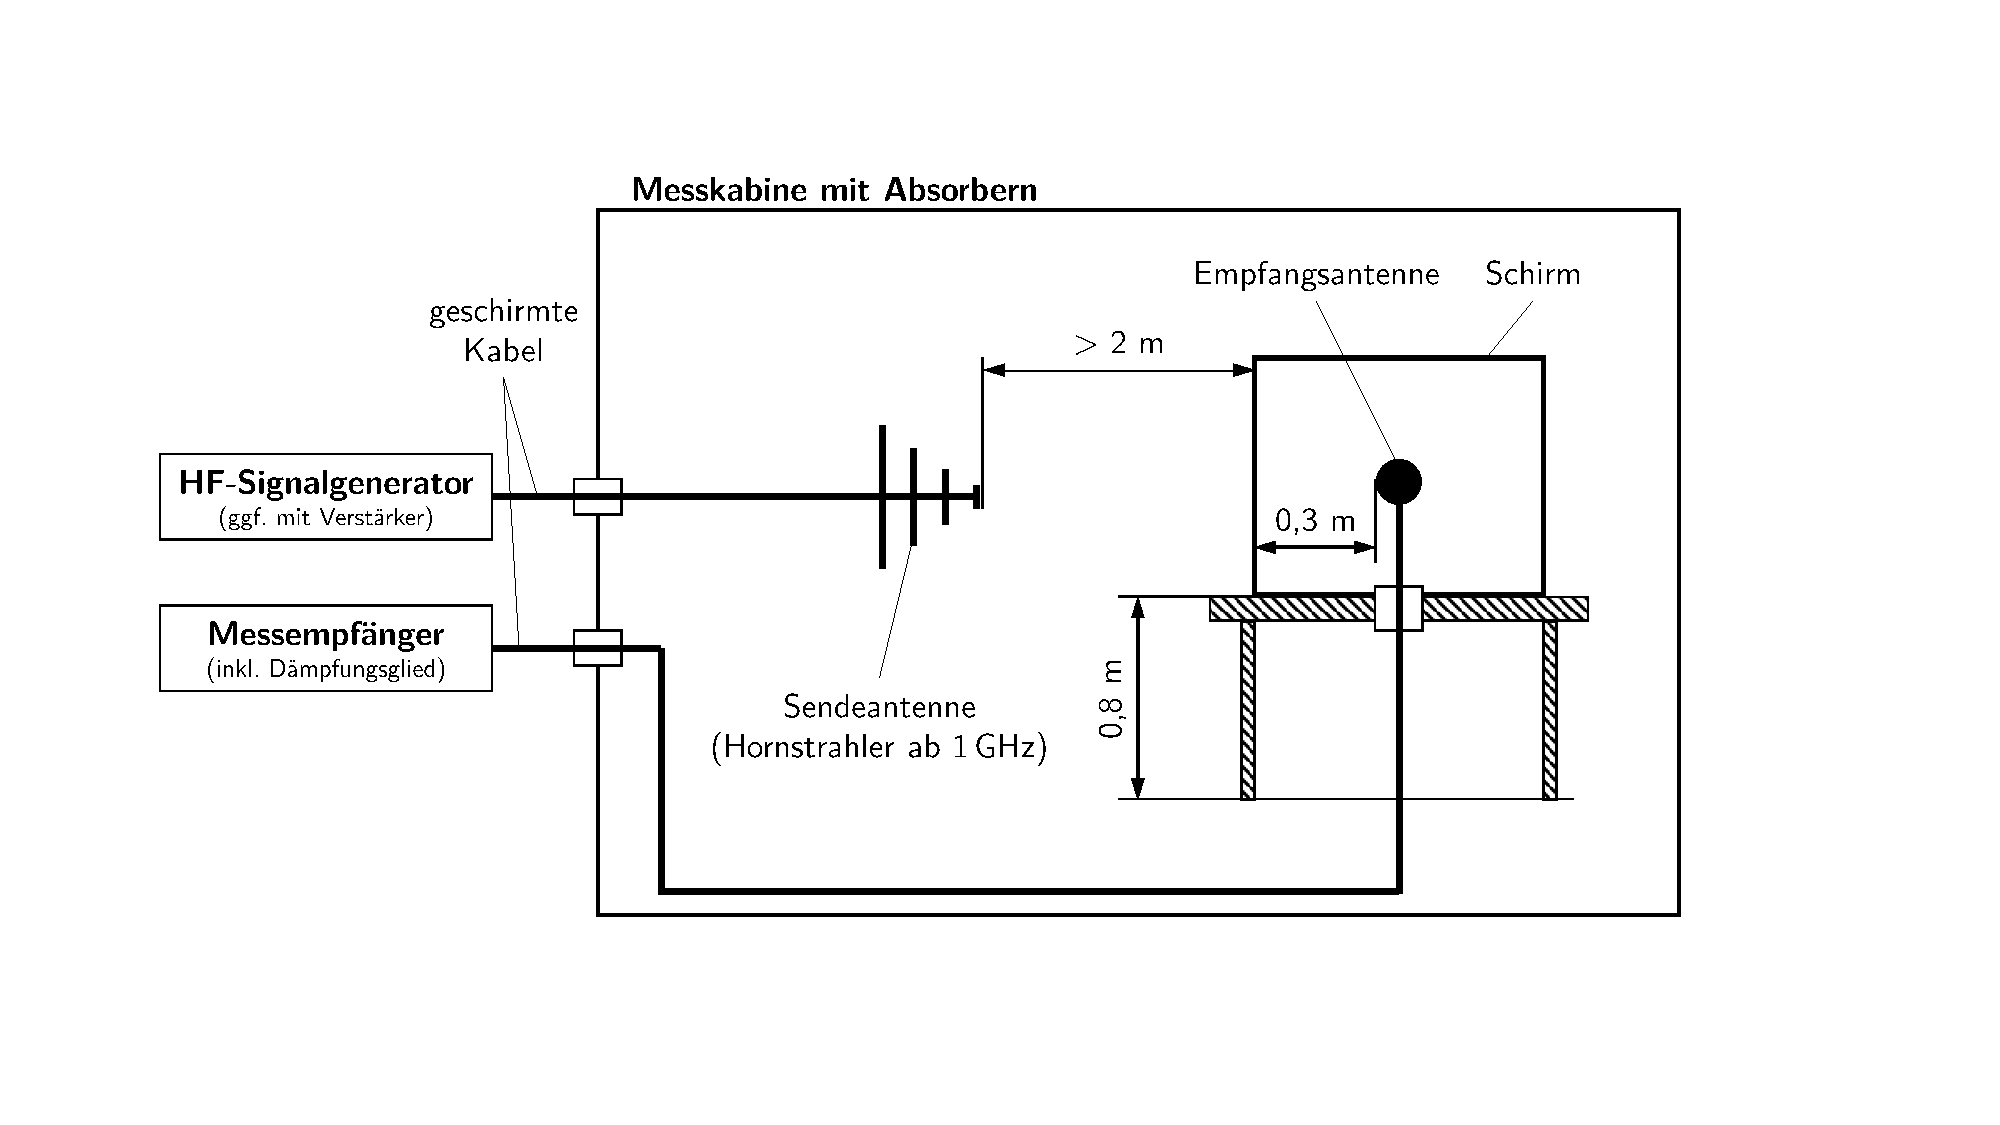
\includegraphics[page = 1, trim = 2cm 3cm 5cm 3cm, clip, width=.9\textwidth]{Abbildungen/Kapitel2/Schematiken_Schirmdaempfungsmessung.pdf}
    \caption[Schematischer Messaufbau der Schirmdämpfungsmessung nach \citeauthor{DIN_EN_61000-5-7} im Frequenzbereich zwischen \SI{1}{\giga\hertz} bis \SI{40}{\giga\hertz}]{Schematischer Messaufbau der Schirmdämpfungsmessung nach \citeauthor{DIN_EN_61000-5-7} im Frequenzbereich zwischen \SI{1}{\giga\hertz} bis \SI{40}{\giga\hertz} nach~\cite{DIN_EN_61000-5-7}}
    \label{fig:2_Schematik_Schirmdaempfungsmessung_DIN_61000-5-7}
\end{figure}


%Anpassung bei hohen Frequenz hinsichtlich Maße

\subsubsection{IEEE 299}
Im Vergleich zur DIN 61000-5-7 soll ebenfalls kurz auf die IEEE 299~\cite{IEEE_299} eingegangen werden, welche die Messung der Schirmdämpfung von Messkabinen und Räumen bis zu einem Frequenzbereich bis \SI{18}{\giga\hertz} beschreibt und den häufig zitierten Standard MIL-STD~285 abgelöst hat~\cite{EM_Schirmung}. Der in \Abb\ref{fig:2_Schematik-Schirmdaempfungsmessung_IEEE_299} gezeigte Messaufbau wird hier sowohl für den Frequenzbereich \SI{20}{\mega\hertz} bis \SI{300}{\mega\hertz}, also auch für den Hochfrequenzbereich ab \SI{300}{\mega\hertz} verwendet, wobei davon ausgagengen wird, dass sich die Schirmung ab \SI{300}{\mega\hertz} im Fernfeld der Antennen befindet und damit nahezu nur ebene Wellen geschirmt werden~\cite{EM_Schirmung, IEEE_299}. In der abgelösten Norm MIL-STD~285 wird im Gegensatz zur echten Einfügungsmessung der IEEE~299 die Empfangsantenne bei sonst ähnlichem Aufbau jeweils vor und hinter dem Schirm platziert~\cite{EM_Schirmung}.
\par
\vspace{\linespace}
Weiterhin beschreibt die DIN~50147"~1~\cite{DIN_EN_50147-1} ein ähnliches Messverfahren zur IEEE~299, jedoch vor allem im Kontext von Absorberhallen.  

\begin{figure}[ht]
    \centering
    \includegraphics[page = 2, trim = 2cm 3cm 4cm 3cm, clip, width=.9\textwidth]{Abbildungen/Kapitel2/Schematiken_Schirmdaempfungsmessung.pdf}
    \caption[Schematischer Messaufbau der Schirmdämpfungsmessung nach \citeauthor{IEEE_299} für Messfrequenzen ab \SI{20}{\mega\hertz}]{Schematischer Messaufbau der Schirmdämpfungsmessung nach \citeauthor{IEEE_299} für Messfrequenzen ab \SI{20}{\mega\hertz} nach~\cite{IEEE_299}}
    \label{fig:2_Schematik-Schirmdaempfungsmessung_IEEE_299}
\end{figure}


\subsection{Modenverwirbelungskammer}
Eine Alternative zur Messung in einer mit Absorbern ausgestatteten Kabine stellt die Messung der Schirmdämpfung in einer Modenverwirbelungskammer~(\acsu{MSC}) dar~\cite{EMV}. Hier werden die Resonanzfrequenzen der Messkabine (vgl. \Abschnitt\ref{cha:2_subsub_Hohlraumresonanzen}) mithilfe beweglicher Metallplattenstrukturen so verändert, dass es im Betrieb nicht zu stehenden Wellen kommt und Hohlraumresonanzen somit nicht auftreten. Dafür müssen jedoch die Kammer und der sogenannte Modenrührer gut aufeinander abgestimmt sein und es muss eine entsprechend hohe Modendichte im gewünschten Messintervall vorliegen. 
\par
\vspace{\linespace}
Bei Schirmdämpfungsmessungen von Gehäusen haben \acp{MSC} den Vorteil der kurzen Messzeit, da eine Drehung des Prüflings nicht notwendig ist, und der guten Vergleichbarkeit, da kleine Unterschiede im Messaufbau nur von geringer Bedeutung sind~\cite{EMV}. Allerdings ist die Auswertung der Messwerte deutlich komplexer und die Feldverteilung ist aufgrund der vielen erzwungenen Reflexionen quasi nicht bestimmbar~\cite{EMV}.  


%siehe EMV 
\subsection{Auswahl der geeigneten Messmethode}
Aufgrund der erwähnten nutzbaren oberen Grenzfrequenz von etwa \SI{1,6}{\giga\hertz} für die Messungen mit TEM-Messzellen sind diese und ähnliche Messaufbauten im Rahmen dieser Arbeit nicht sinnvoll nutzbar. Weiterhin überwiegen für den vorliegenden Anwendungsfall auch bei \acp{MSC} die erwähnten Nachteile, sodass diese als Konzept für die zu entwickelnde Messkammer ebenfalls verworfen wurden. 
\par
\vspace{\linespace}
Die Messung in einer Absorberkammer durch Einfügung der Prüflinge in die Signalstrecke zweier Antennen in Anlehnung an~\cite{DIN_EN_61000-5-7, IEEE_299} stellt somit nach dem betrachteten Stand der Wissenschaft die beste Methode zur Ermittlung der Schirmdämpfung von Materialproben im Fernfeld dar. Im folgenden Kapitel~\ref{cha:3} wird der gewählte Aufbau im Detail dargelegt.







%Entscheidung für Absorberkammer mit Reflektor (ähnlich wie in Textil-Quelle) und Maßen in Anlehnung an Norm  



